\section{Simulation}

A realistic model of the LTCC has been developed, describing the location and material composition
of the support box, the mirrors, photo-multipliers, Winston Cones, magnetic shields and the $C_4F_{10}$ gas.

A 3D view of the simulated geometry of the LTCC \F{simOverview}. The LTCC GEMC simulation software details are summarized in the simulation article of this volume.


\begin{figure}
	\centering
	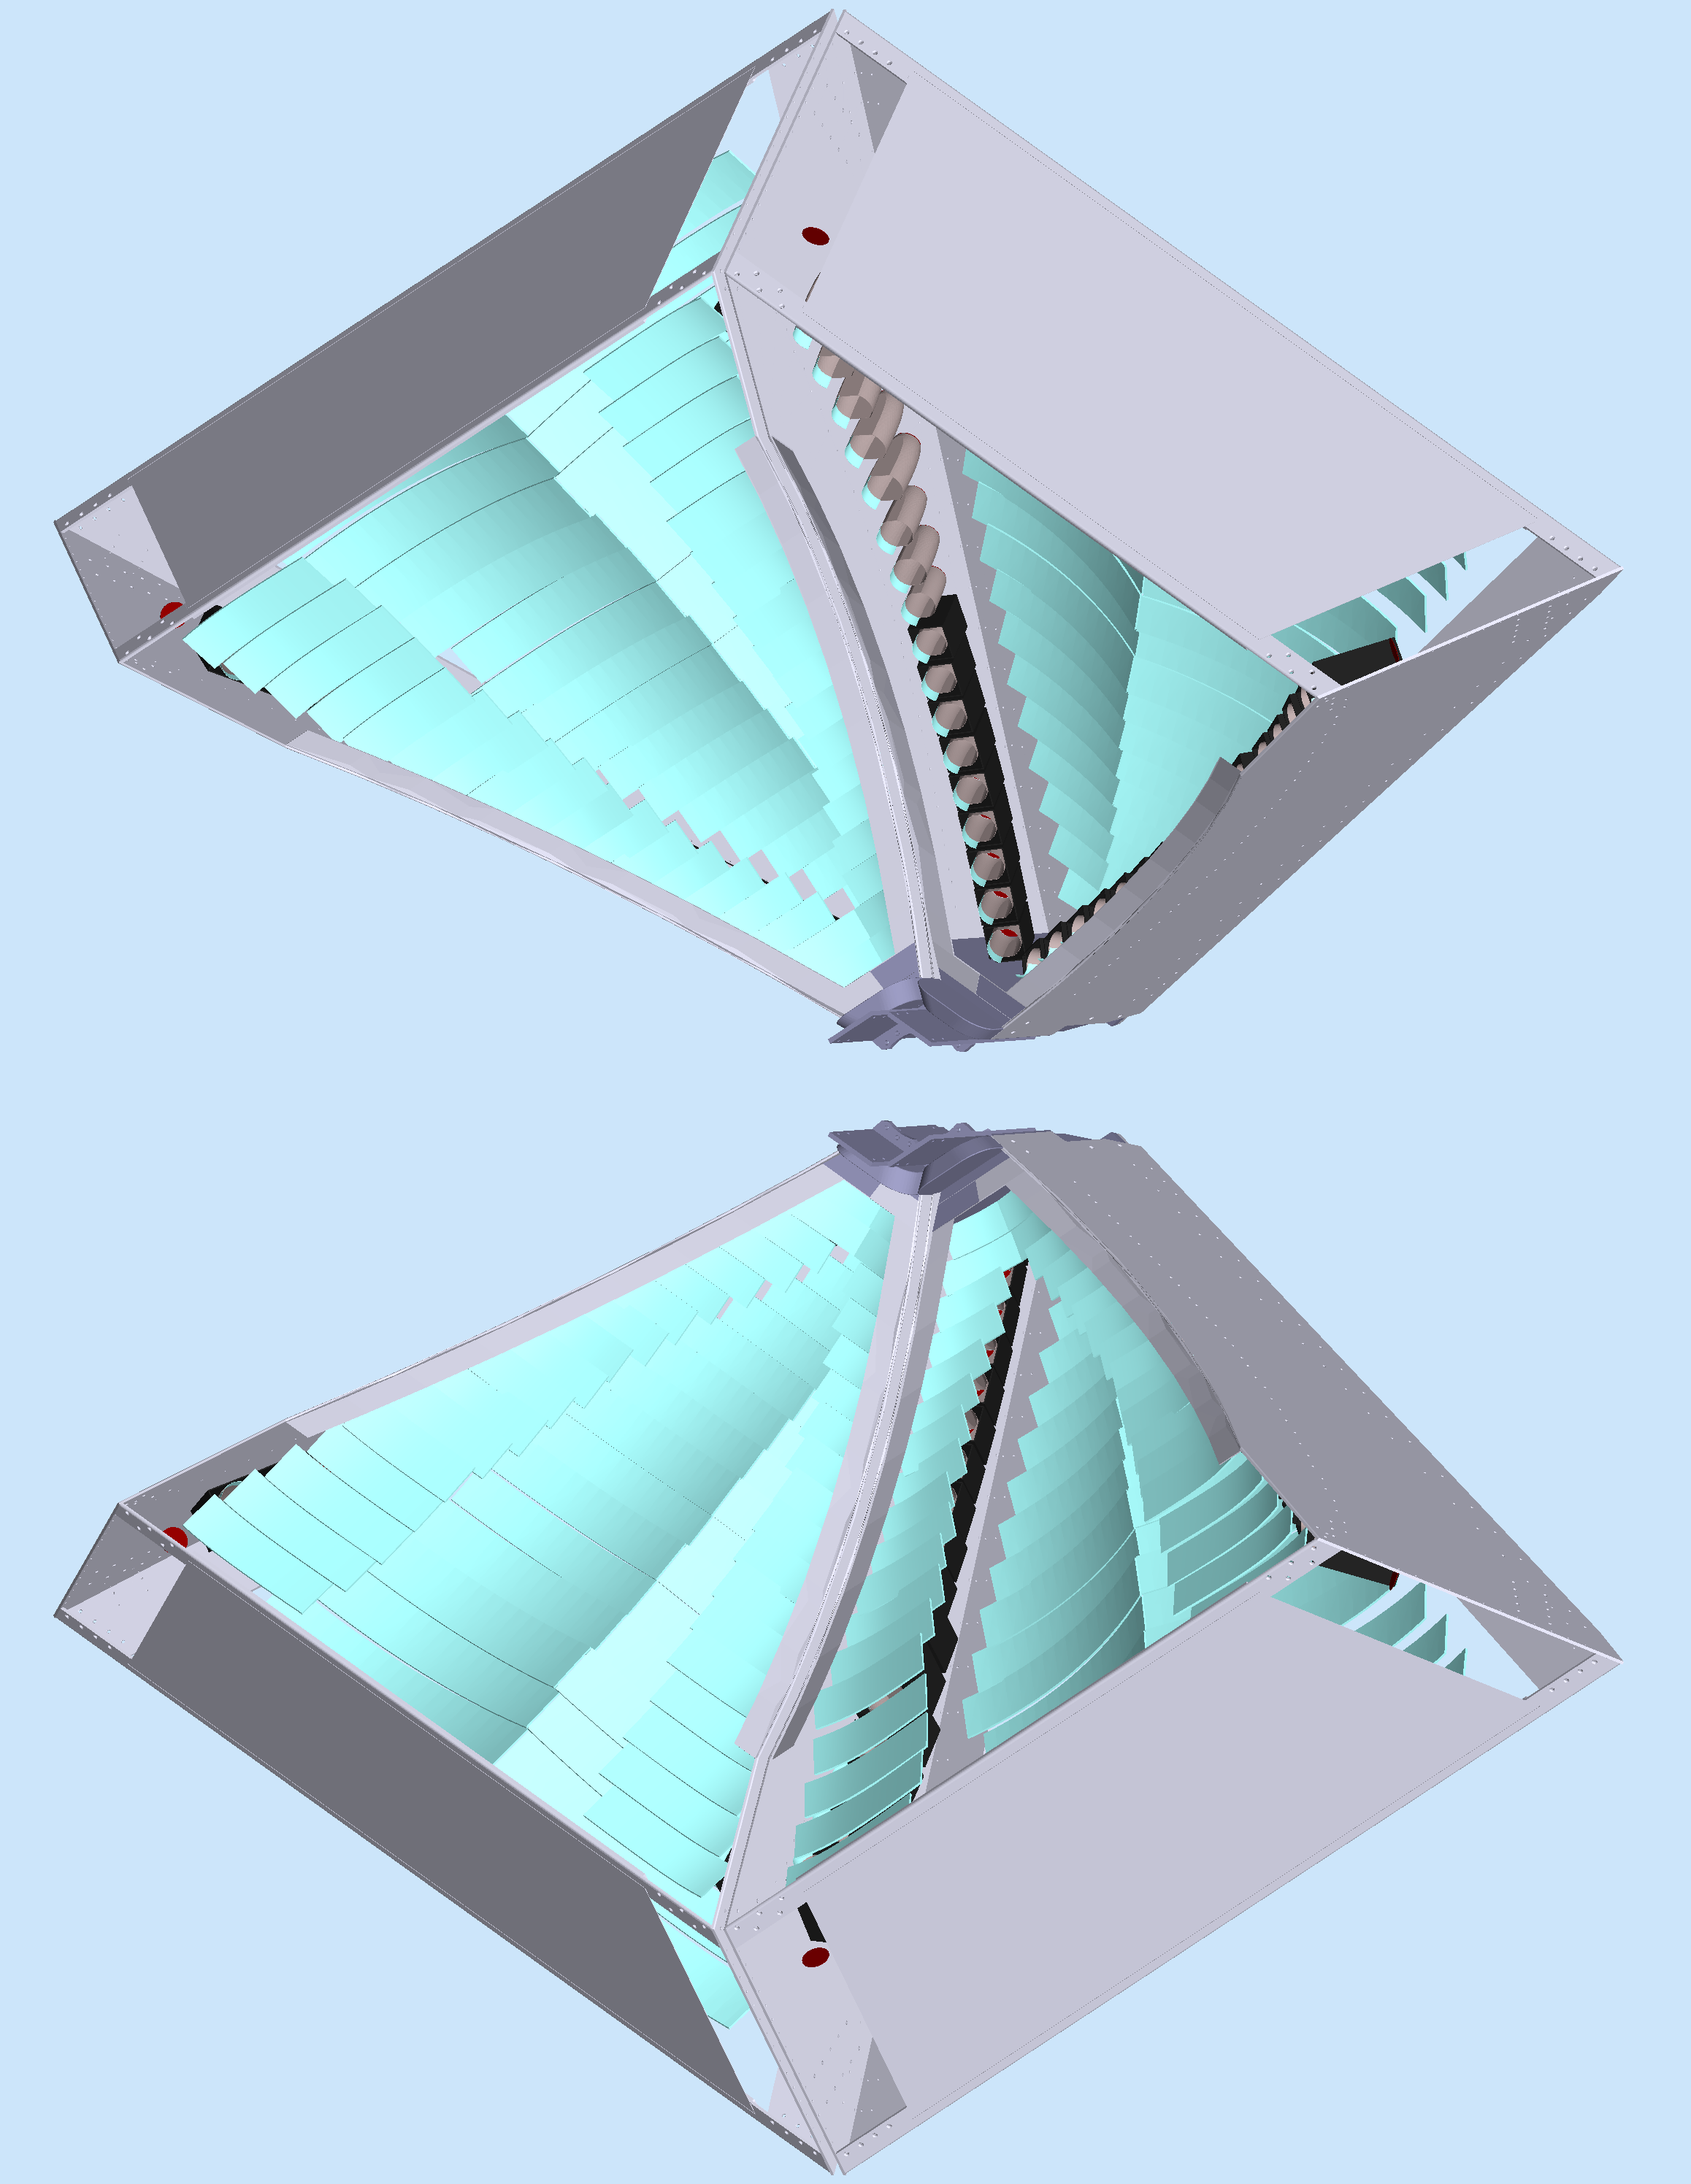
\includegraphics[width=0.95\columnwidth,keepaspectratio]{img/simOverview.png}
	\caption{The geant4 model of the LTCC implemented in GEMC. This view correspond to the Run Group A CLAS12 experiments
				where the LTCC sectors 2, 3, 5 and 6 were present. In this picture the hyperbolic mirrors and some magnetic shields
            in sector3 (upper right) have been made transparent to show details of the Winston Cones (grey) and magnetic shields (black).}
	\label{fig:simOverview}
\end{figure}

\subsection{Mirrors Geometry}

The Cherenkov light is emitted on a small cone around the direction of the emitting particle. The angle of
incidence of the particles entering the LTCC can be different from the angle at the production vertex due to the bending of the tracks
inside the toroidal magnetic field. Instead of having two sets of mirrors, one aligned for positive-bending and one aligned for negative-bending particles,
the optics of the mirrors was designed to maximize the light collection of optical photons originating from the target (placed on the center of the CLAS12 coordinate system),
to average the cases for the two charged particles.

The mirror shapes were described mathematically by ellipsoid and hyperbolic curves.
The ellipsoid first focal point is the target location and the second focal point was chosen
to place the mirrors as far back in the box as possible to maximize the amount og gas seen by the tracks.
The second ellipsoid focal point overlaps with the hyperbolic first focal point. The hyperbole shape was optimized to focus the light
collection on PMTs placed on the shadow of the torus magnet coil, near the LTCC box walls, see \F{mirrorMath}.


\begin{figure}
	\centering
	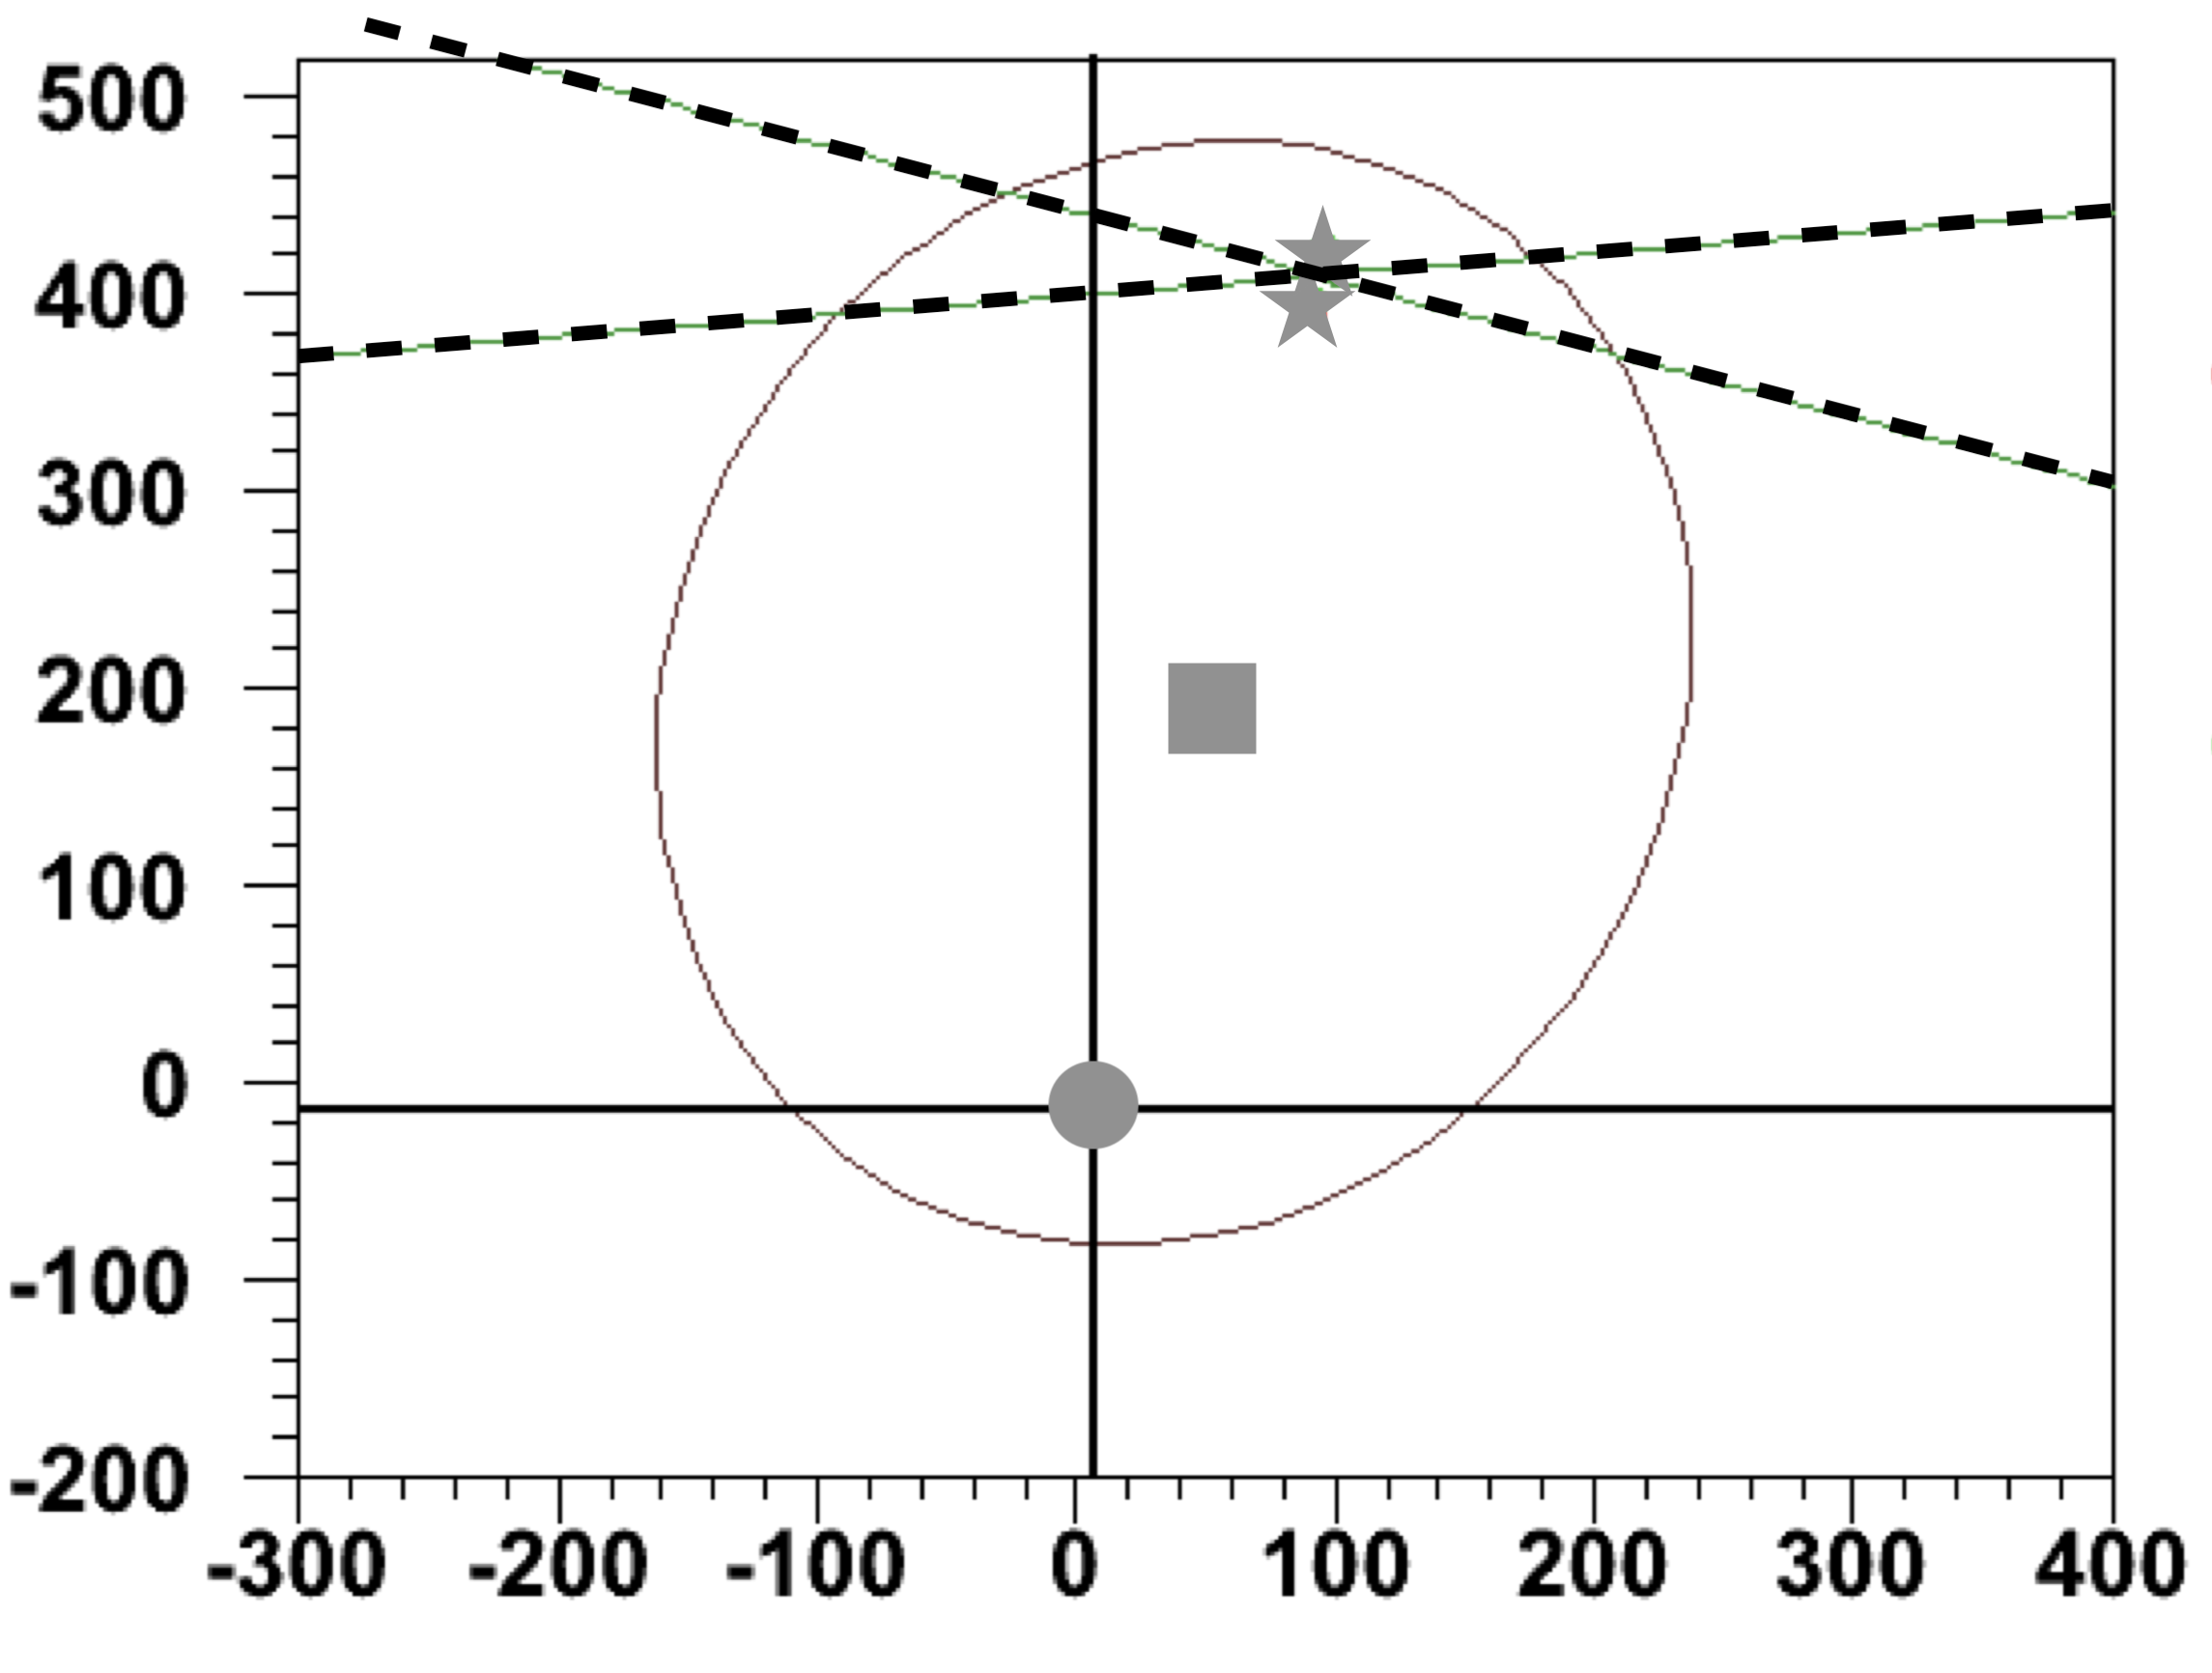
\includegraphics[width=0.95\columnwidth,keepaspectratio]{img/mirrorMath1.png}
	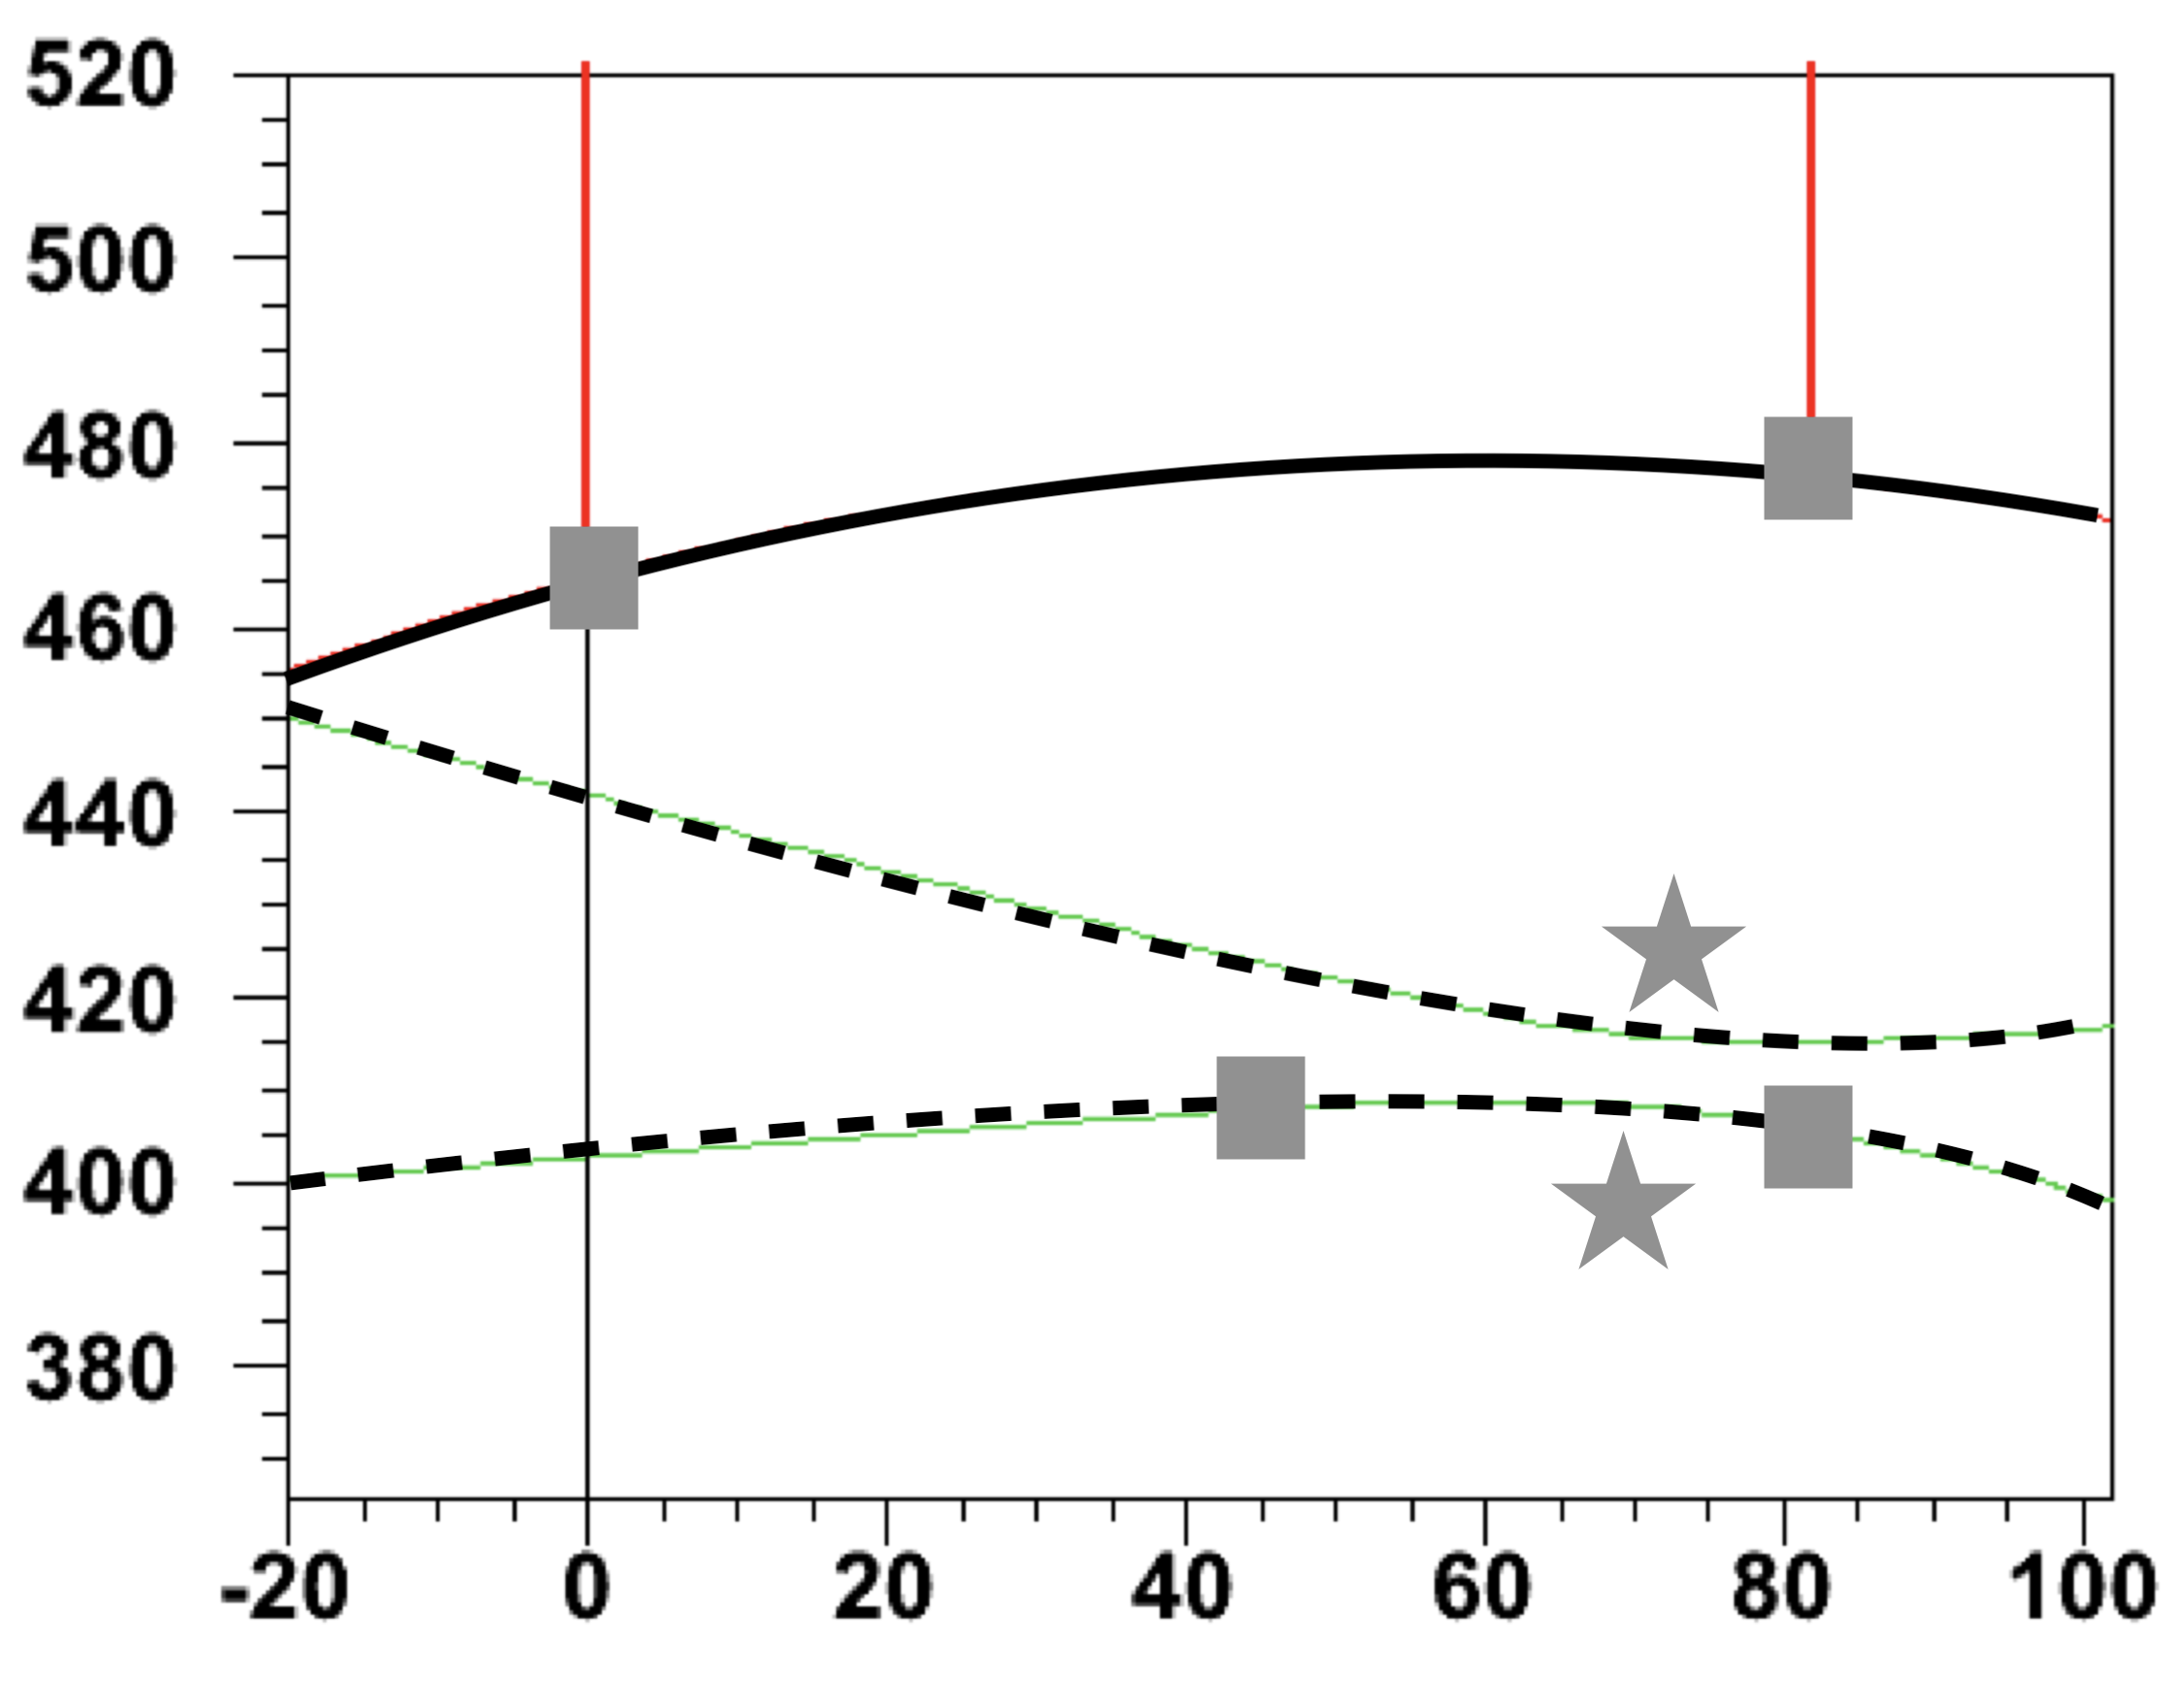
\includegraphics[width=0.95\columnwidth,keepaspectratio]{img/mirrorMath2.png}
	\caption{Top: The ellipsoid shape (black line), with its center (red diamond) and the two focal points (red circles). The two hyperbolas
			   that have the corresponding focal points (green circles) are the green curves. Bottom: details of the mirrors azimuthal limits: the triangles represent
            the elliptical mirror left and right edges. The crosses are the hyperbolical mirrors edges. All these parameters are stored in databases and
            loaded in the software modeling the LTCC mirrors in the GEMC simulation.}
	\label{fig:mirrorMath}
\end{figure}

In the geant4 implementation the elliptical mirrors are composed by, for each segment:

\begin{enumerate}
	\item ellipse shells: the subtraction of two ellipsoidal volumes, rotated and centered on their designed position for the mirrors on the right side of the box.
	\item ellipse azimutal slices: subraction of the shells with left and right boxes to ``cut'' the mirrors left and right edges
	\item placed mirrors: the resulting volumes,  are then copied to their left side of the box counterpart.
\end{enumerate}

The hyperbolic mirrors are made by polycon that approximate the mathematical shape of the mirrors using a number of faucets
varying from 10 (smallest mirror) to 30 faucets (longest mirrors).


\subsection{Winston Cones Geometry}


\subsection{Box Support Structure}

support structure in active area  + nose

\subsection{PMTs and Shields}

pmts shields

\subsection{Digitizations}

spe at 200 + sigmas
pmts q.e.
output

\subsection{Run Period Variations}


variations for run periods



